\documentclass{ctexbeamer}
\usetheme[red]{sjtubeamer}
\usesjtutheme{poster}
% \usesjtutheme[landscape]{poster}
% \usesjtutheme[sepinst]{poster}
% \usesjtutheme[noindent]{poster}
\usepackage{subcaption}
\usepackage[style=gb7714-2015]{biblatex}
\addbibresource{\getcontribpath{poster}{ref.bib}}
\usepackage{zhlipsum}
\begin{document}
% 当标题较长时,可以使用 \\ 换行。
\title{poster 子主题\\使用说明}
\author{作者}
\logo{\zhlogo}
\institute[Test Institute]{测试机构}
\footline[左脚注]{右脚注}
\begin{frame}[fragile]
  \begin{columns}[T]
    \begin{column}{.45\textwidth}

      \begin{stampblock}{主题概述}
        \texttt{poster} 子主题基于 \texttt{beamerposter} 宏包\cite{beamerposter},对
        SJTUBeamer 进行适配以制作海报,展示您的成果。
        \codeblockinput[firstline=1,lastline=3]{开始使用}{poster.tex}
      \end{stampblock}

      \begin{stampblock}{风格建议}
        建议使用 \texttt{stampblock} 环境分割不同的区块。你也可以使用 \texttt{block}
        环境分割不同的区块。相较于普通 \texttt{beamer} 幻灯片文字较少的情形,\texttt{poster}
        更有可能会写入大段文字,所以默认情况下这些区块内部会有首行缩进。由于 \texttt{column}
        环境内部不受外部首行缩进的影响,所以不推荐之间在
        \texttt{column} 环境中书写内容,而应该再套一层 \texttt{stampblock} 或 \texttt{block}。

        可以插入图片来丰富你的海报内容,但请注意由于海报的纸张尺寸较大,像一些高 DPI
        显示的场景一样,会对文字大小进行缩放,但是度量上却没有发生变化,请注意要使用相对于平时更大的度量插入图片。

        不推荐直接插入 Ti\emph{k}Z 的代码,推荐使用 \texttt{standalone} 文档类产生 PDF
        文件后再插入,否则会导致图片内的文字过大而排版错乱。
      \end{stampblock}

      \begin{stampblock}{多栏对齐}
        推荐使用 \texttt{columns} 环境分割多栏,环境可选选项可以用于指定顶部对齐 \texttt{t},居中对齐
        \texttt{c},底部对齐 \texttt{b}。

        \codeblockinput[firstline=16,lastline=16,firstnumber=1]{多栏}{poster.tex}
      \end{stampblock}

    \end{column}
    \begin{column}{.45\textwidth}

      \begin{stampblock}{图文混排}
        由于 \texttt{beamer} 关闭了浮动体浮动,所以推荐使用多栏分割的方式实现图文混排。
        或者是多图并排放置。
        \begin{columns}
          \begin{column}{0.7\textwidth}
            上海交通大学的东大门---紫气东来门,简称庙门,位于上海市闵行区莲花南路 4800 号。
          \end{column}
          \begin{column}{0.3\textwidth}
            \begin{figure}
              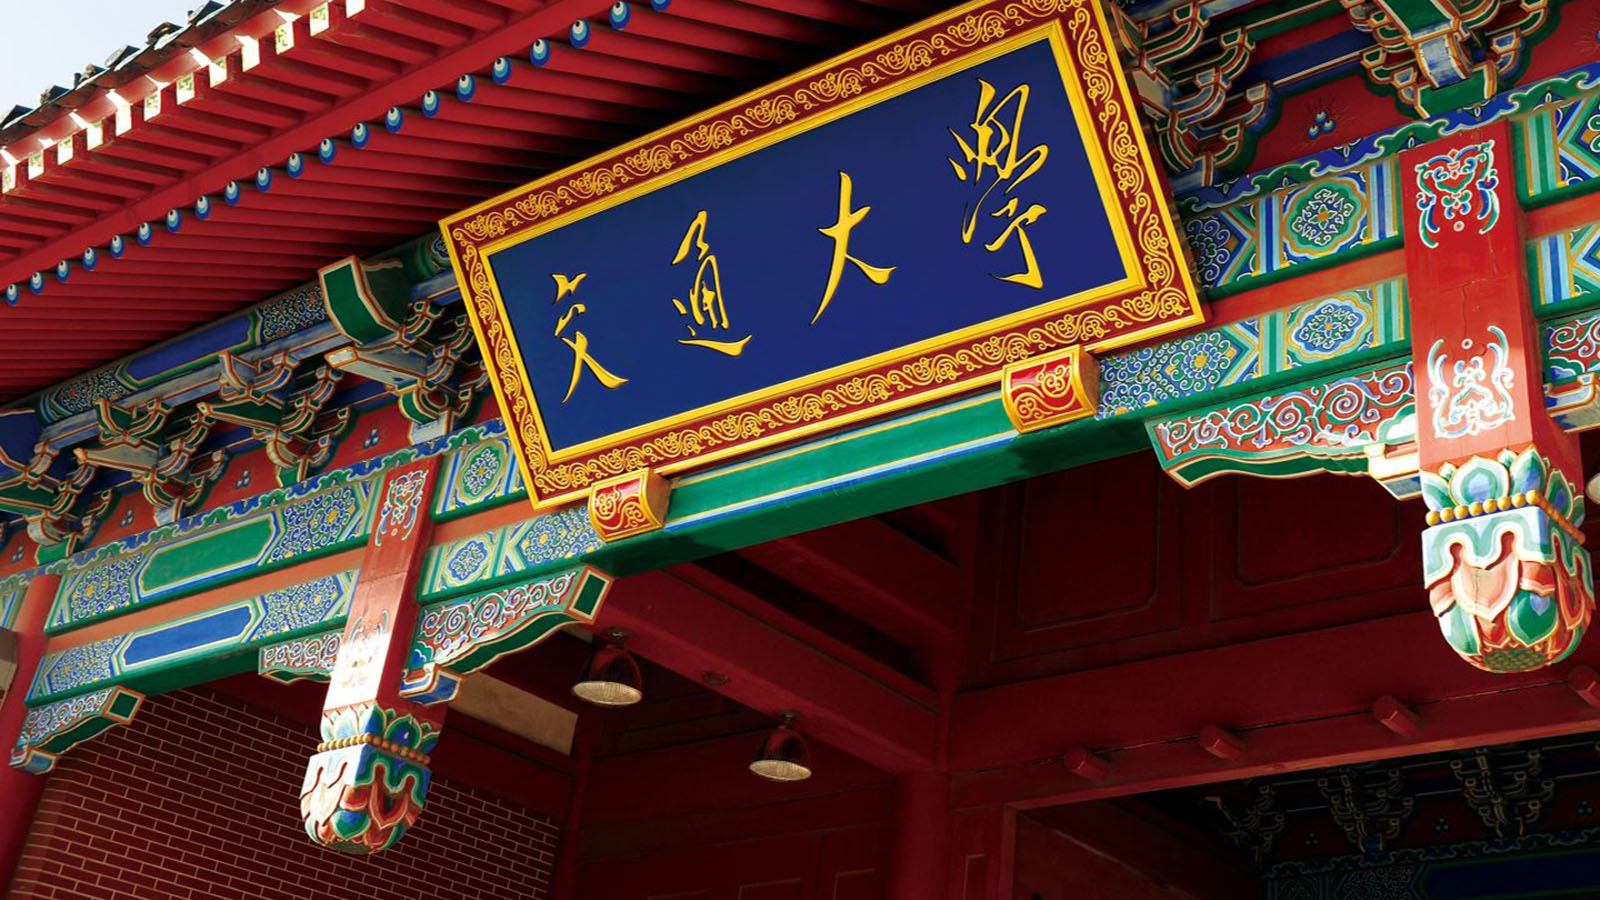
\includegraphics[width=\textwidth]{vi/sjtu-vi-sjtuphoto.jpg}
              \caption{庙门}
            \end{figure}
          \end{column}
        \end{columns}
        \begin{figure}
          \begin{subfigure}{0.4\textwidth}
            \resizebox{\textwidth}{!}{\secondaryinstlogo[Test
                Institute]{测试机构}{\zhlogo}}
            \caption{中文}
          \end{subfigure}\hspace*{20pt}
          \begin{subfigure}{0.4\textwidth}
            \resizebox{\textwidth}{!}{\secondaryinstlogo[]{Test
                Institute}{\enlogo}}
            \caption{英文}
          \end{subfigure}
          \caption{二级机构徽标}
        \end{figure}
      \end{stampblock}

      \begin{stampblock}{参考文献}

        可以使用图标样式的参考文献。

        \begin{bibliolist}{00}
          \onlineitem \textsc{Tantau T}, \textsc{Wright J}, and
          \textsc{Mileti\'c V}.\newblock
          The beamer class: User Guide for version 3.67[OL].\newblock
          2022. \url{https://github.com/josephwright/beamer}
          \articleitem \textsc{上海交通大学}.\newblock
          上海交通大学视觉形象识别系统[OL].\newblock
          2016. \url{https://vi.sjtu.edu.cn}
          \bookitem \textsc{Knuth DE}.\newblock
          The \TeX{}book[M].\newblock
          Addison-Wesley. 1986.
        \end{bibliolist}

        你也可以使用 \texttt{biblatex} 插入参考文献。

        \printbibliography

      \end{stampblock}

    \end{column}
  \end{columns}

  % 正文中的分割线使用 \posterstamphrule
  \posterstamphrule[cprimary]

  \begin{columns}
    \begin{column}{0.45\textwidth}
      \begin{block}{选项}
        \texttt{poster} 子主题拥有一些选项。
        \begin{description}
          \item[\texttt{sepinst}] 分离徽标与机构于两侧
          \item[\texttt{landscape}] 横向海报
          \item[\texttt{noindent}] 首行不缩进
        \end{description}
      \end{block}
      \begin{alertblock}{脚注}
        使用 \texttt{\textbackslash{}footline[左脚注]\{右脚注\}} 设定左脚注和右脚注。
      \end{alertblock}
      \begin{exampleblock}{区块}
        仍然可以使用内置的 \texttt{block}, \texttt{alertblock}, \texttt{exampleblock}
        插入对应的区块。
      \end{exampleblock}
    \end{column}
    \begin{column}{0.45\textwidth}

      \begin{stampblock}[a]{印记区块}
        使用 \texttt{stampblock} 环境插入带有印记图案的区块,编号会自动递增。你也可以通过指定可选参数来设置编号内容。
      \end{stampblock}

      \begin{codeblock}[numbers=none]{代码块}
% 应当减少代码块的使用,增加了标题栏的高度。
% 关闭代码行号编号可以在 codeblock 上添加选项 numbers=none
      \end{codeblock}

      \begin{columns}[b]
        \begin{column}{.5\textwidth}
          \begin{stampbox}
            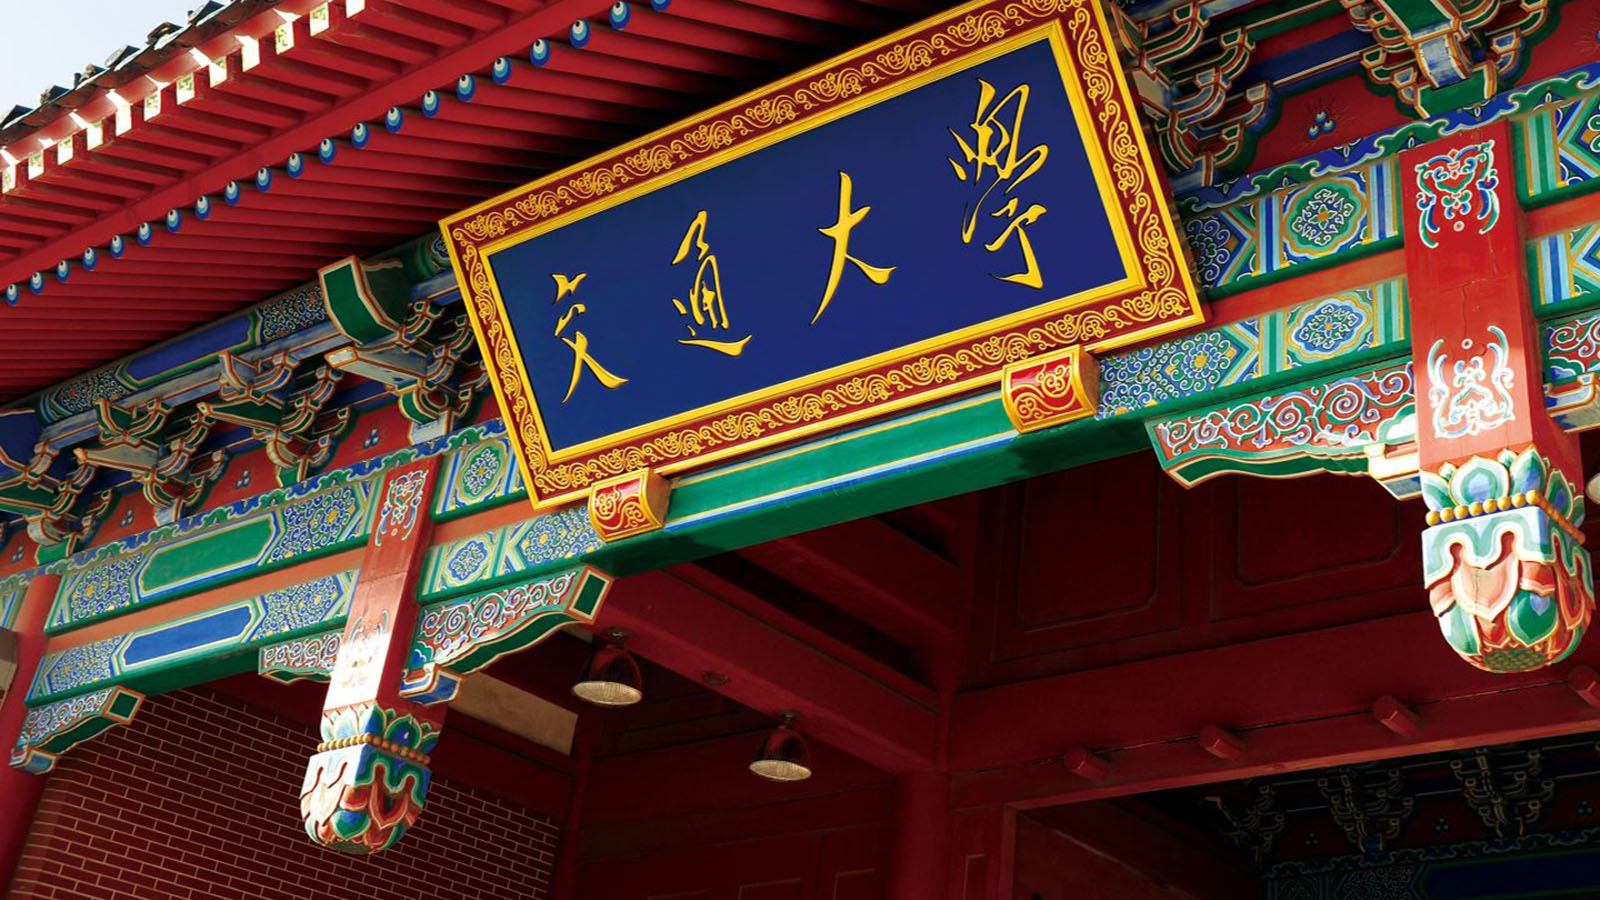
\includegraphics[width=16cm]{vi/sjtu-vi-sjtuphoto.jpg}
          \end{stampbox}
        \end{column}
        \begin{column}{.5\textwidth}
          $\leftarrow$ 你仍然可以使用 \texttt{stampbox} 环境插入带边框的图片\vspace{1ex}
          % column 环境中的分割线仍然使用 \stamphrule
          \stamphrule
        \end{column}
      \end{columns}
    \end{column}
  \end{columns}
\end{frame}
\title{}
\author{}
\logo{}
\institute[]{}
\begin{frame}
  \begin{columns}

    \begin{column}{.5\textwidth}
      \begin{stampblock}{测试}
        \zhlipsum[1]
      \end{stampblock}

      \begin{stampblock}{测试}
        \zhlipsum[2]
      \end{stampblock}

      \vspace*{0.5ex}

      \begin{stampblock}{测试}
        \zhlipsum[3]
      \end{stampblock}
    \end{column}

  \end{columns}

\end{frame}
\end{document}